\problemname{Röknet}

Inni í hverri tölvu má finna svokölluð \emph{röknet}. Þessi net eru notuð til
að reikna gildi röksegða, og mynda því grunninn að flóknari reikningum sem
tölvan framkvæmir. Röknet samanstanda af mismunandi gerðum af hlutum sem geta
haft allt að tvo innganga og allt að einn útgang. Hlutur tekur sanngildi inn
um þessa innganga, framkvæmir einhverja einfalda reglu til að búa til nýtt
sanngildi, og sendir það svo út um útganginn. Þessa hluti er svo hægt að tengja
saman þannig að útgangur á einum hlut er tengdur við inngang á öðrum hlut.
Hlutirnir mynda því net sem sanngildi ferðast í gegnum.

Í þessu verkefni ætlum við að skoða fimm gerðir af hlutum:
\begin{itemize}
\item \texttt{OG} rökhlið hefur tvo innganga. Ef báðir inngangarnir eru sannir, þá er satt sent út um útganginn, en ósatt annars.
\item \texttt{EDA} rökhlið hefur tvo innganga. Ef báðir inngangarnir eru ósannir, þá er ósatt sent út um útganginn, en satt annars.
\item \texttt{EKKI} rökhlið hefur einn inngang. Ef inngangurinn er sannur, þá er ósatt sent út um útganginn, en satt annars.
\item \texttt{INNTAK} hefur engan inngang en einn útgang. \texttt{INNTAK} er sérstakur hlutur sem notaður er til að senda alltaf sama sanngildið út um útganginn.
\item \texttt{UTTAK} hefur einn inngang en engan útgang. \texttt{UTTAK} er sérstakur hlutur sem notaður er til að skoða hvaða sanngildi kemur inn um innganginn.
\end{itemize}

Í eftirfarandi mynd sjáum við dæmi um svona röknet.

\begin{figure}[h]
    \centering
    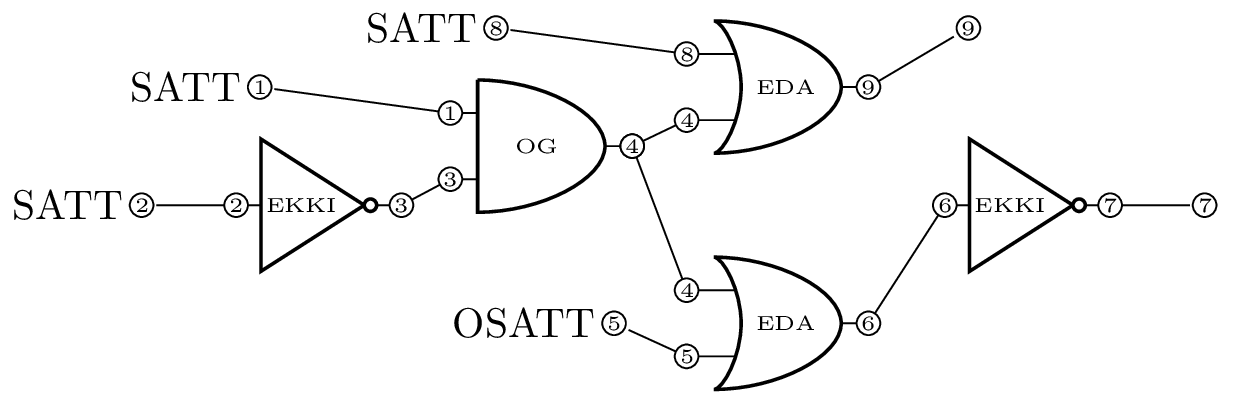
\includegraphics[width=0.8\textwidth]{network.png}
    \caption{Mynd af fyrsta sýnidæminu}
\end{figure}

Gefin lýsing á svona rökneti, getur þú reiknað hvaða sanngildi koma í \texttt{UTTAK} hlutina?

\section*{Inntak}
Á fyrstu línu er jákvæða heiltalan $N$ sem táknar fjölda hluta í
röknetinu. Svo fylgja $N$ línur, ein fyrir hvern hlut. Það eru fimm gerðir af
línum eftir því um hvers konar hlut er að ræða:
\begin{itemize}
\item \texttt{INNTAK \textit{nafn} \textit{sanngildi}} táknar hlut af gerðinni \texttt{INNTAK} að nafni \textit{nafn} sem sendir sanngildið \textit{sanngildi} út um útganginn.
\item \texttt{UTTAK \textit{inn}} táknar ónefndan hlut af gerðinni \texttt{UTTAK}. Inngangur hlutarins er tengdur við útgang hlutarins að nafni \textit{inn}.
\item \texttt{OG \textit{inn1} \textit{inn2} \textit{nafn}} táknar \texttt{OG} rökhlið að nafni \texttt{nafn}. Inngangar rökhliðsins eru tengdir við útganga hlutanna sem heita \textit{inn1} og \textit{inn2}.
\item \texttt{EDA \textit{inn1} \textit{inn2} \textit{nafn}} táknar \texttt{EDA} rökhlið að nafni \texttt{nafn}. Inngangar rökhliðsins eru tengdir við útganga hlutanna sem heita \textit{inn1} og \textit{inn2}.
\item \texttt{EKKI \textit{inn} \textit{nafn}} táknar \texttt{EKKI} rökhlið að nafni \texttt{nafn}. Inngangur rökhliðsins er tengdur við útgang hlutarins að nafni \textit{inn}.
\end{itemize}

Nafn hlutanna eru mismunandi og samanstanda af enskum lágstöfum og tölustöfum.
Ef útgangur hlutar $A$ er tengdur við inngang hlutar $B$, þá mun hlutur $A$
vera skilgreindur í inntakinu áður en hlutur $B$ er skilgreindur í inntakinu.

\section*{Úttak}
Fyrir hvern hlut af gerð \texttt{UTTAK} á að skrifa út eina línu með nafninu á
inngangnum og sanngildinu sem kemur inn um innganginn; \texttt{SATT} ef það er
satt, \texttt{OSATT} ef það er ósatt. Þessar línur eiga að koma í sömu röð og
hlutirnir af gerð \texttt{UTTAK} eru skilgreindir í inntakinu.

\section*{Stigagjöf}
Lausnin mun verða prófuð á miserfiðum inntaksgögnum, og er gögnunum skipt í
hópa eins og sýnt er í töflunni að neðan. Lausnin mun svo fá stig eftir því
hvaða hópar eru leystir.

\begin{tabular}{|l|l|l|l|}
\hline
Hópur & Stig & Inntaksstærð & Önnur skilyrði \\ \hline
1 & 20 & $N \leq 100$ & Eingöngu hlutir af gerðinni \texttt{INNTAK} og \texttt{UTTAK} \\ \hline
2 & 30 & $N \leq 100$ & \\ \hline
3 & 50 & $N \leq 10^4$ & \\ \hline
\end{tabular}
